\chapter{Introduction}

What was/is the purpose of this thesis? Why did we develop these computational simulations? Really, we need a goal!

In this thesis, a lattice Monte Carlo approach was used to simulate diffusion. Also used a finite difference method to simulate diffusion. Both problems were boundary-value problems.

We also performed an analysis: MSD, mean position, etc.?? Analysis is kind of empty!

Overall overview to thesis? What kind of an overview? Or just a general background to some main concepts needed or used in this thesis? How does this compare with the abstract?
	
\section{Diffusion}
Say something general 

\section{Monte Carlo Simulations}


\section{Finite Difference (Master Equation) Simulations}
This was done is 1D and 2D.

\section{Simple Cell Model}

Nearly all human cells are microscopic in size; their diameters range from 7.5 \si{\micro\meter} to approximately 150 \si{\micro\meter} and a cell exhibits a particular size or shape that reflects the specific task it's designated to perform. There are many different types of cells including nerve cells, muscle cells, and gland cells, but despite their anatomical and functional differences, the cells of the human body have many similarities. It is a fact that no cell contains all cellular components found in all the cell types, so often a \textit{composite cell} is used to exhibit the most important characteristics. Each cell is enclosed by a plasma membrane that separates the cell from the surrounding environment. The inside of the cell is largely composed of a gel-like substance that is dense arrangement of proteins, organelles, and other molecules, suspended in a watery fluid called cytosol. The dense crowding of molecules and organelles results in frequent physical interactions, therefore promoting metabolic efficiency \citep{ap}.


\begin{figure}[h]
	\centering
	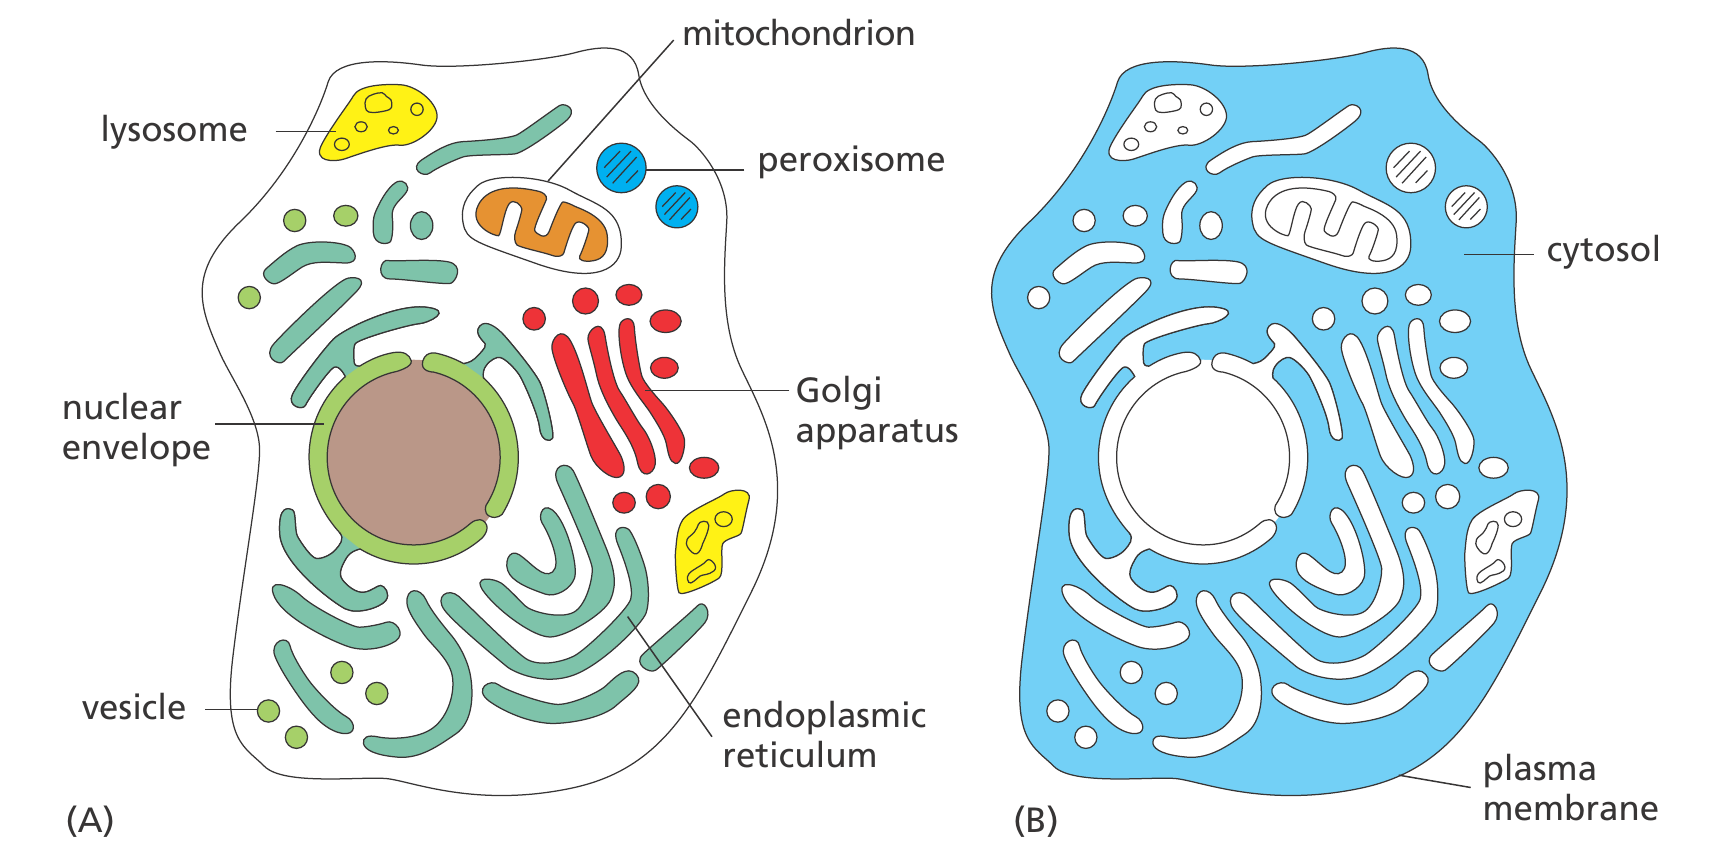
\includegraphics[width=1.0\linewidth]{cellpic_2.png}
	\caption{Composite cell showing various important and common internal cell structures. Most of the volume within the cell is occupied by the cytosol fluid.}
	\label{fig:group2_object2_side2_pulses13(edited)}
\end{figure}


In a multicellular organism, there are several levels of biological organization. A cell is the lowest level of organization that is considered living; tissues are the next higher level of organization and are composed of cells similar in structure and function. This ensemble of cells resides in an extracellular matrix (ECM); a medium containing water, fibrous and adhesive proteins, glycoproteins, and other molecules. The ECM varies in composition between different tissues, but providing structural support and facilitating cell-to-cell communication are common functions of the ECM.Normally, the cytoplasm is more viscous than the extracellular matrix. \citep{cr-biology}.






















\section{A sample introduction}

This is just an example, but I wanted to show you some common things to do with Latex.

\subsection{A subsection example}

For of all, here's an equation -- it's the NFW formula, given by \citet{nfw95}, and looks like
\begin{equation}
	\label{eq:nfw}
	\rho(r) = \frac{\rho_s}{r / r_s (1 + r / r_s)^2},
\end{equation}
where $\rho_s$ and $r_s$ are a characteristic density and scale radius, respectively.

Now, I can reference that equation later, since it's labelled properly; it's equation (\ref{eq:nfw}).  Notice that I cited a paper above; I could do that in a different way like this \citep{nfw95}.

Just one other quick thing:  figures.  There's one below, and again it's properly labelled.  It's Figure \ref{fig:intro_density}.

\begin{figure}
\begin{center}
	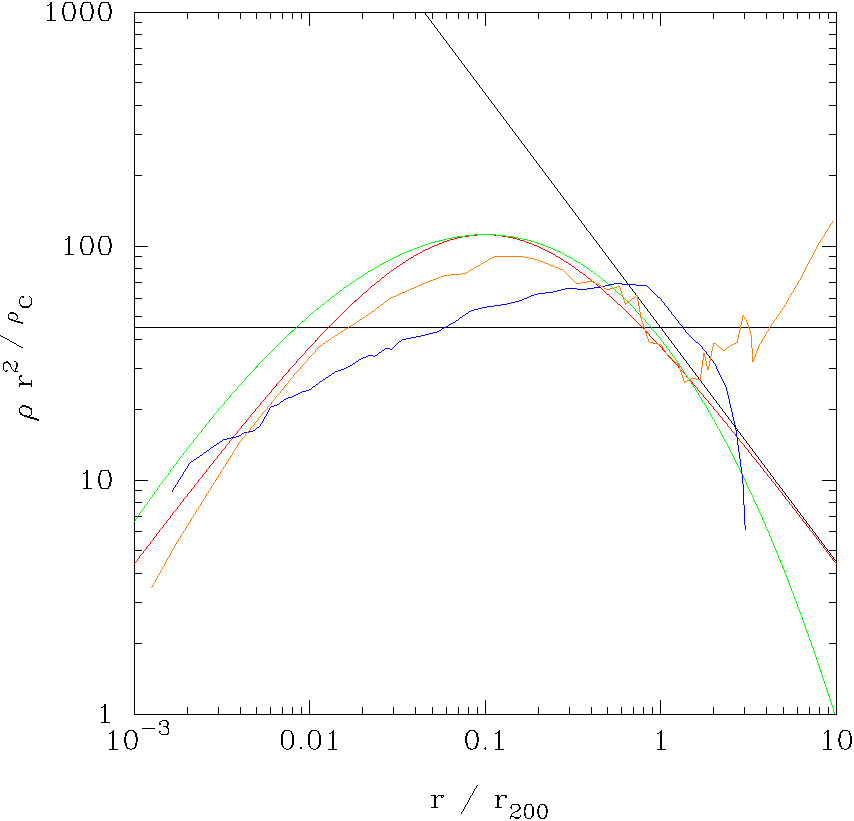
\includegraphics[scale=0.8]{intro_density.pdf}
\end{center}
	\caption[Density profiles of various models]{Density profiles, shown as $\rho r^2$ to better highlight the differences, of various models.  }
	\label{fig:intro_density}
\end{figure}